\newpage
\thispagestyle{empty}
\section{Контрольная работа 2}

\subsection[2018-2019]{\hyperref[sec:sol_kr_02_2018_2019]{2018-2019}}
\label{sec:kr_02_2018_2019}

\begin{enumerate}

    %Задача 1
    \item В шляпе лежат четыре игральные карты: тройка, семерка, туз и пиковая дама. Наудачу из шляпы извлекается одна карта. Рассмотрим две случайные величины
\[
    \xi = \left\{
                \begin{array}{ll}
                    1, & \text{если выпал туз,} \\
                    0, & \text{в противном случае,}
            \end{array}
            \right.
\]
\[
    \eta = \left\{
                \begin{array}{ll}
                    1, & \text{если выпала пиковая дама,} \\
                    0, & \text{в противном случае.}
            \end{array}
            \right.
\]
\begin{enumerate}
  \item Составьте таблицу совместного распределения случайных величин $\xi$ и $\eta$ (3 балла)
\newline Найдите
  \item $\E(\xi)$ и $\E(\eta)$ (1 балл)
  \item $\Cov(\xi, \, \eta)$ (2 балла)
  \item $\P\bigl(\xi = 1 | \eta = 0\bigr)$ и $\P\bigl(\xi = 0 | \eta = 0\bigr)$ (1 балл)
  \item $\E\bigl(\xi | \eta = 0 \bigr)$ (1 балл)
  \item Постройте таблицу распределения случайной величины $\E(\xi|\eta)$ (3 балла)
\end{enumerate}
    %Задача 2
    \item В финал по стрельбе из лука вышло два лучника. Лучник зарабатывает одно очко, если попадает в яблоко с $20$ метров. Первый лучник попадает с вероятностью $0.5$, а второй — с вероятностью $0.6$. Каждый стрелок делает по 50 выстрелов. Победившим считается стрелок, который наберет большее число очков. Используя центральную предельную теорему найдите вероятность того, что
\begin{enumerate}
  \item Первый стрелок заработает не менее 15 очков (5 баллов)
  \item Победит первый стрелок (7 баллов)
\end{enumerate}


    %Задача 6
    \item Вася ходит обедать в студенческую столовую. В среднем на обед он тратит 300 рублей со стандартным отклонением 30 рублей. Оцените сверху вероятность того, что
    \begin{enumerate}
    \item Вася потратит на обед более тысячи рублей (2 балла)
\item Сумма, потраченная Васей на обед, будет отличаться от 300 рублей более, чем на 100 рублей (3 балла)
\end{enumerate}

    %Задача 7
    \item Чтобы добраться до Вышки Вася едет на трамвае. Время ожидания трамвая $T_{1}$ и время поездки на трамвае $T_{2}$ — независимые случайные величины, равномерно распределенные на отрезке $[0,20]$ и $[10,20]$ минут. Найдите:

    \begin{enumerate}
    \item Математическое ожидание и дисперсию общего времени поездки $T_{1}+T_{2}$ (3 балла)
    \item Вероятность того, что Вася доберётся до Вышки не более, чем за 15 минут (4 балла)
    \item Плотность распределения общего времени поездки $T_{1}+T_{2}$ (7 баллов)
\end{enumerate}

%Задача 3
    \item Пусть $\xi_1, \, \xi_2, \, \xi_3$ — независимые стандартные нормальные случайные величины и $\eta = \xi_1 \, \xi_2 \, \xi_3$. Найдите
\begin{enumerate}
  \item $\E(\eta)$ (2 балла)
  \item $\Var(\eta)$ (3 балла)
  \item $\P(e^{\xi_1} < 1)$ (3 балла)
\end{enumerate}

    %Задача 5
    \item Сибирский крокодил Утундрий решил заняться риск-менеджментом. В этот раз он изучает теорию эффективных портфелей ценных бумаг. Пусть $R_1$, $R_2$ и $R_3$ — доходности трёх ценных бумаг. Утундрий обладает следующей информацией:
\[
    \E(R_1) = 5, \;\;\; \E(R_2) = 10, \;\;\; \E(R_3) = 15,
\]
\[
    \Var(R_1) = 50, \;\;\; \Var(R_2) = 100, \;\;\; \Var(R_3) = 150,
\]
\[
    \Cov(R_1, \, R_2) = 20, \;\;\; \Cov(R_1, \, R_3) = -10, \;\;\; \Cov(R_2, \, R_3) = -10.
\]
Крокодил Утундрий знает, что $w_1$, $w_2$ и $w_3$, доли первой, второй и третьей ценных бумаг в портфеле, неотрицательны и в сумме дают единицу, а кроме того:
\begin{itemize}
  \item \textit{доходность} этого портфеля вычисляется по формуле $R : = w_1 \, R_1 + w_2 \, R_2 + w_3 \, R_3$,
  \item \textit{ожидаемая доходность} этого портфеля есть $\E(R)$,
  \item \textit{риск} данного портфеля определяется как $\sqrt{\Var(R)}$.
\end{itemize}

Утундрий составил два портфеля $A$ и $B$. Доли ценных бумаг, которые входят в портфель $A$ задаются вектором $w_A = (1/2, \, 1/2, \, 0)$, а в портфель $B$ — вектором $w_B = (0, \, 1/2, \, 1/2)$.
Помогите Утундрию ответить на следующие вопросы.
\begin{enumerate}
  \item Найдите ожидаемые доходности портфелей $A$ и $B$ (1 балл)
  \item Найдите риски портфелей $A$ и $B$ (3 балла)
  \item Какой из портфелей $A$ или $B$ имеет большую ожидаемую доходность, а какой — меньший риск (1 балл)
  \item Найдите коэффициент корреляции между доходностями портфелей $A$ и $B$ (4 балла)
  \item Предложите собственный портфель (доли $w_{1}$, $w_{2}$ и $w_{3}$) обладающий доходностью не меньшей, чем портфели $A$ и $B$, но меньшим риском (5 баллов)
\end{enumerate}

\begin{figure}[h]
    \noindent\centering{
    
\includegraphics[width=80mm]{images/utundri.jpg}
    }
    \caption{Утундрий!}
    \label{ut2018}
\end{figure}


    %Задача 8
    \item Для произвольно выбранного студента вероятность того, что он «дойдёт» до устной части экзамена по Теории Вероятностей составляет 0.1. Время ответа (в часах) на устном части подчинено показательному распределению с параметром 2. Для курса из 300 человек найдите математическое ожидание совокупного времени ответов студентов на устном экзамене (6 баллов).

    \textbf{Подсказка}: Если случайная величина $V$ – число студентов, пришедших на устный экзамен, а $\tau_{i}$ — время ответа $i$-го студента, то требуется найти $\E(\tau_{1}+\tau_{2}+ \ldots +\tau_{V})$.


\end{enumerate}

\subsection[2017-2018]{\hyperref[sec:sol_kr_02_2017_2018]{2017-2018}}
\label{sec:kr_02_2017_2018}

\subsubsection*{Минимум}
% 2 + 4 + 14 + 16

\begin{enumerate}
\item Приведите определение условной вероятности случайного события, формулу Байеса.
\item Сформулируйте определение и свойства функции плотности случайной величины.
\item Сформулируйте определение  условного математического ожидания $\E(Y|X=x)$ для совместного дискретного и совместного абсолютно непрерывного распределений.
\item Сформулируйте неравенство Чебышёва и неравенство Маркова.

\item Задана таблица совместного распределения случайных величин $X$ и $Y$.
\begin{center}
\begin{tabular}{lccc}
\toprule
                      & $Y=-1$  & $Y=0$   & $Y=1$   \\ \midrule
$X=0$                 & $0.2$ & $0.1$ & $0.3$ \\
$X=1$                 & $0.2$ & $0.1$ & $0.1$ \\
\bottomrule
\end{tabular}
\end{center}

\begin{enumerate}
    \item Найдите $F_{X,Y}(0, 0)$;
    \item Найдите $\E(X)$, $\E(X^2)$, $\E(Y)$, $\E(Y^2)$;
    \item Найдите $\Var(X)$, $\Var(Y)$;
    \item Найдите $\Cov(X, Y)$, $\Corr(X, Y)$
\end{enumerate}

\item Плотность распределения случайного вектора $(X,Y)$ имеет вид
\[
f_{X,Y}(x,y) =
\begin{cases}
\frac{4x+10y}{7}, & \text{при } (x,y) \in [0;1] \times [0;1] \\
0 , & \text{при } (x,y) \not\in [0;1] \times [0;1] \\
\end{cases}
\]
\begin{enumerate}
\item Найдите $\P(X \leq Y)$;
\item Найдите функцию плотности $f_X(x)$;
\item Найдите $\E(X)$, $\E(Y)$ и $\Cov(X, Y)$;
\item Являются ли случайные величины $X$ и $Y$ независимыми?
\end{enumerate}
\end{enumerate}

\subsubsection*{Задачи}

\begin{enumerate}[resume]

\item Статистика авиакомпании «А» за много лет свидетельствует о том, что 10\% людей, купивших билет на самолет, не являются на рейс. Авиакомпания продала 330 билетов на 300 мест.
\begin{enumerate}
\item Какова вероятность, что всем явившимся на рейс пассажирам хватит места?
\item Укажите наибольшее число билетов, которое можно продавать на 300 мест, чтобы случаи переполнения случались не чаще, чем на одном из десяти рейсов.
\end{enumerate}

\item Сегодня акция компании «Ух» стоит 1 рубль. Каждый день акция может с вероятностью 0.7 вырасти на 1\%, с вероятностью 0.2999 упасть на 1\% и с вероятностью 0.0001 обесцениться (упасть на 100\%).
\begin{enumerate}
\item Считая изменение цены акции независимыми, найдите математическое ожидание её стоимости через 20 торговых дней.
\item Найдите предел по вероятности среднего изменения цены акции в процентах на бесконечном промежутке времени (Ответ обоснуйте).
\item Найдите математическое ожидание цены акции на бесконечном промежутке времени.
\item Инвестор вложил все свои средства в акции компании «Ух». Найдите вероятность его разорения на бесконечном промежутке времени.
\end{enumerate}
\end{enumerate}



\newpage
\subsection[2016-2017]{\hyperref[sec:sol_kr_02_2016_2017]{2016-2017}}
\label{sec:kr_02_2016_2017}

\textbf{Неравенства Берри–Эссеена:} Для любых $n \in \mathbb{N}$ и всех
$x \in \mathbb{R}$ имеет место оценка:
\[
\bigl|F_{S_n^{*}}(x) - \Phi(x)\bigr| \leq 0.48 \cdot \frac{\E(|\xi_i - \E\xi_i|^3)}{\Var^{3/2}(\xi_i)\cdot\sqrt{n}} \text{,}
\]
где $\Phi(x) = \int_{-\infty}^{x}\frac{1}{\sqrt{2\pi}}e^{-\frac{t^2}{2}}\,dt$, \; $S_n^* = \frac{S_n - \E(S_n)}{\sqrt{\Var(S_n)}}$, \; $S_n = \xi_1 + \ldots + \xi_n$

\textbf{Распределение Пуассона:} Случайная величина $\xi$ имеет распределение Пуассона
с параметром $\lambda > 0$,  если она принимает целые неотрицательные значения с
вероятностями $\P(\{\xi = k\}) = \frac{\lambda^k}{k!}e^{-\lambda}$. Приличным
студентам должно быть известно, что в этом случае $\E(\xi) = \Var(\xi) = \lambda$.

\begin{enumerate}
\item Пусть $\E(\xi) = 1$, $\E(\eta) = -2$, $\Var(\xi) = 1$, $\E(\eta^2) = 8$, $\E(\xi \eta) = -1$. Найдите
\begin{enumerate}
\item $\E(2\xi-\eta+1)$, $\Cov(\xi, \,\eta)$, $\Corr(\xi, \,\eta)$,  $\Var(2\xi-\eta+1)$;
\item $\Cov(\xi+\eta, \,\xi+1)$, $\Corr(\xi+\eta, \,\xi+1)$, $\Corr(\xi+\eta-24, \,365 - \xi - \eta)$, $\Cov(2016\cdot\xi, \, 2017)$.
\end{enumerate}

\item
Совместное распределение доходностей акций двух компаний задано с помощью таблицы:

\begin{center}
\begin{tabular}{ccc}
\toprule
         & $\eta=-1$ & $\eta=1$ \\ \midrule
$\xi=-1$  & $0.1$       & $0.2$ \\
$\xi=0$   & $0.2$       & $0.2$ \\
$\xi=2$   & $0.2$       & $0.1$ \\
\bottomrule
\end{tabular}
\end{center}

\begin{enumerate}
  \item Найдите частные распределения случайных величин $\xi$ и $\eta$.
  \item Найдите $\Cov(\xi,\,\eta)$.
  \item Сформулируйте определение независимости дискретных случайных величин.
  \item Являются ли случайные величины $\xi$ и $\eta$ независимыми?
  \item Найдите условное распределение случайной величины $\xi$, если $\eta = 1$.
  \item Найдите условное математическое ожидание случайной величины $\xi$, если $\eta = 1$.
  \item Найдите математическое ожидание и дисперсию величины $\pi = 0.5\, \xi + 0.5\, \eta$.
  \item Рассмотрим портфель, в котором $\alpha$ — доля акций с доходностью $\xi$
  и $(1 - \alpha)$ — доля акций с доходностью $\eta$. Доходность этого портфеля
  есть случайная величина
  \[
  \pi(\alpha) = \alpha \xi + (1-\alpha)\eta.
  \]
  Найдите такую долю $\alpha \in [0;\,1]$, при которой доходность портфеля $\pi(\alpha)$
  имеет наименьшую дисперсию.
\end{enumerate}

\item Число посетителей сайта \url{pokrovka11.wordpress.com} за один день имеет
распределение Пуассона с математическим ожиданием 250.
\begin{enumerate}
  \item Сформулируйте неравенство Маркова. При помощи данного неравенства оцените
  вероятность того, что за один день сайт посетят более 500 человек.
  \item Сформулируйте неравенство Чебышева. Используя данное неравенство, определите
  наименьшее число дней, при котором с вероятностью не менее 99\% среднее за день
  число посетителей будет отличаться от 250 не~более чем на 10.
  \item Решите предыдущий пункт с помощью центральной предельной теоремы.
  \item Сформулируйте закон больших чисел. Обозначим через $\xi_i$ число посетителей
  сайта за $i$-ый день. Найдите предел по вероятности последовательности
  $\frac{\xi_1^2 + \ldots + \xi_n^2}{n}$ при $n \rightarrow \infty$.
\end{enumerate}

\item Отведав медовухи, Винни–Пух совершает случайное блуждание на прямой. Он
стартует из начала координат и в каждую следующую минуту равновероятно совершает
шаг единичной длины налево или направо. Передвижения Винни-Пуха схематично
изображены на следующем рисунке.
\begin{figure}[h]
    \noindent\centering{
    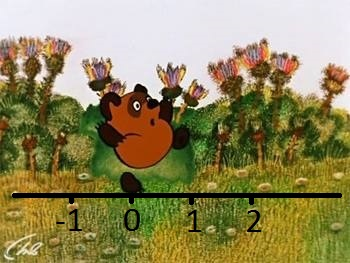
\includegraphics[width=80mm]{images/Winnie_the_Pooh_and_Medovuh.jpg}
    }
    \caption{Случайные бродилки.}
    \label{wun762hkej}
\end{figure}
\begin{enumerate}
  \item Сформулируйте центральную предельную теорему.
  \item При помощи центральной предельной теоремы оцените вероятность того, что
  ровно через час блужданий Винни-Пух окажется в области $(-\infty; \, -5]$.
  \item Используя неравенство Берри–Эссеена оцените погрешность вычислений предыдущего
  пункта.
\end{enumerate}

\item
Cлучайные величины $\xi$ и $\eta$ означают время безотказной работы рулевого
управления и двигателя автомобиля соответственно. Время измеряется в годах.
Совместная плотность имеет вид:
\[
f_{\xi, \,\eta}(x,\,y) =
\begin{cases}
0.005\,e^{-0.05\,x-0.1\,y} & \text{ при } x > 0, y > 0, \\
0                    & \text{ иначе.}
\end{cases}
\]

\begin{enumerate}
  \item Найдите частные плотности распределения случайных величин $\xi$ и $\eta$.
  \item Являются ли случайные величины $\xi$ и $\eta$ независимыми?
  \item Найдите вероятность того, что двигатель прослужит без сбоев более пяти лет.
  \item Найдите вероятность того, что двигатель прослужит без сбоев более восьми лет,
  если он уже проработал без сбоев три года.
  \item Найдите условное математическое ожидание безотказной работы рулевого управления,
  если двигатель проработал без сбоев пять лет,  $\E(\xi | \eta = 5)$.
  \item Найдите вероятность того, что рулевое управление проработает без сбоев на
  два года больше двигателя, $\P(\{\xi - \eta > 2\})$.
\end{enumerate}

\item Бонусная задача

Случайная величина $\xi$ имеет плотность распределения
\[
f_{\xi}(x) = \frac{1}{2} \cdot \frac{1}{\sqrt{2\pi}}e^{-\frac{(x-1)^2}{2}} + \frac{1}{2} \cdot \frac{1}{\sqrt{2\pi}}e^{-\frac{(x+1)^2}{2}} \text{.}
\]

\begin{enumerate}
\item Найдите $\E(\xi)$, $\E\left(\xi^2\right)$, $\Var(\xi)$.
\item Покажите, что функция $f_{\xi}(x)$, действительно, является плотностью распределения.
\end{enumerate}
\end{enumerate}



\newpage
\subsection[2015-2016]{\hyperref[sec:sol_kr_02_2015_2016]{2015-2016}}
\label{sec:kr_02_2015_2016}

\begin{enumerate}
\item Функция плотности случайного вектора $\xi=(\xi_1, \xi_2)^T$ имеет вид
\[
f(x,y)=\begin{cases}
0.5x + 1.5y, \text{ если } 0<x<1, \; 0<y<1 \\
0, \text{ иначе }
\end{cases}
\]
Найдите:
\begin{enumerate}
\item Математическое ожидание $\E(\xi_1 \cdot \xi_2)$
\item Условную плотность распределения $f_{\xi_1|\xi_2} (x|y)$
\item Условное математическое ожидание $\E(\xi_1| \xi_2=y)$
\item Константу $k$, такую, что функция $h(x,y)=kx\cdot f(x,y)$ будет являться
совместной функцией плотности некоторой пары случайных величин
\end{enumerate}

\item На курсе учится очень много студентов. Вероятность того, что случайно
выбранный студент по результатам рубежного контроля имеет хотя бы один незачет
равна $0.2$. Пусть $\xi$ и $\eta$ — число студентов с незачетами и без незачетов
в случайной группе из $10$ студентов. Найдите $\Cov(\xi,\eta)$, $\Corr(\xi,\eta)$,
$\Cov(\xi-\eta,\xi)$. Являются ли случайные величины $\xi-\eta$ и $\xi$ независимыми?

\item Доходности акций компаний А и В – случайные величины $\xi$ и $\eta$. Известно,
что $\E(\xi)=1$, $E(\eta)=1$, $\Var(\xi)=4$, $\Var(\eta)=9$, $\Corr(\xi,\eta)=-0.5$.
Петя принимает решение потратить свой рубль на акции компании А, Вася — 50 копеек
на акции компании А и 50 копеек на акции компании В, а Маша  принимает решение
вложить свой рубль в портфель $R=\alpha\xi+(1-\alpha)\eta$, $(0 \leq \alpha \leq 1)$,
обладающий минимальным риском. Найдите $\alpha$, ожидаемые доходности и риски портфелей
Пети, Васи и Маши.

\item Будем считать, что рождение мальчика и девочки равновероятны.
\begin{enumerate}
\item Оцените с помощью неравенства Маркова вероятность того, что среди тысячи
новорожденных младенцев, мальчиков будет более 75\%.
\item Оцените с помощью неравенства Чебышёва вероятность того, что доля мальчиков
среди тысячи новорожденных младенцев будет отличаться от $0.5$ более, чем на $0.25$
\item С помощью теоремы Муавра-Лапласа вычислите вероятность из предыдущего пункта.
\end{enumerate}

\item Сейчас валютный курс племени «Мумба» составляет 100 оболов за один рубль.
Изменение курса за один день — случайная величина $\delta_i$ с законом распределения:

\begin{center}
\begin{tabular}{lrrr}
\toprule
$x$ & $-1$ & $0$ & $2$ \\
$\P(\delta_i = x)$ & $0.25$ & $0.5$ & $0.25$ \\
\bottomrule
\end{tabular}
\end{center}

Найдите вероятность того, что через полгода (171 день) рубль будет стоить более
250 оболов, если ежедневные изменения курса происходят независимо друг от друга.

\item \textbf{Бонусная задача}

Число посетителей, зашедших в магазин в течении дня — пуассоновская случайная
величина с параметром $\lambda$. Каждый из посетителей совершает покупку с
вероятностью $p$, не зависимо от других посетителей. Найдите математическое ожидание
числа человек, совершивших покупку.
\end{enumerate}



\newpage
\subsection[2014-2015]{\hyperref[sec:sol_kr_02_2014_2015]{2014-2015}}
\label{sec:kr_02_2014_2015}

\begin{enumerate}
\item Ежемесячные расходы студенческой семьи Маши и Васи хорошо описываются случайным
вектором $(X,Y)$, ($X$ — расходы Маши, $Y$ — расходы Васи), имеющим равномерное
распределение в треугольнике, задаваемом ограничениями $\{0 \leq X, \; 0\leq Y,
\; X+Y \leq 1 \}$.

Найдите:

\begin{enumerate}
\item Вероятность того, что совокупные расходы превысят половину бюджета, $\P(X+Y>1/2)$
\item Плотность распределения расходов Васи.
\item Вероятность того, что Машины расходы составили менее трети бюджета, если
известно, что Вася израсходовал более половины семейного бюджета.
\item Условную плотность распределения и условное математическое ожидание расходов Маши,
при условии, что Вася израсходовал половину бюджета.
\item Математическое ожидание условного математического ожидания расходов Маши,
$\E(\E(X|Y))$
\item Коэффициент корреляции расходов Маши и Васи
\end{enumerate}

\item Задана последовательность независимых случайных величин $X_1$, $X_2$, \ldots

\begin{center}
\begin{tabular}{llll}
\toprule
$x_n$ & $-\sqrt{n}$ & $0$ & $\sqrt{n}$ \\
$\P(X_n = x_n)$ & $1/2n$ & $1-1/n$ & $1/2n$ \\
\bottomrule
\end{tabular}
\end{center}

\begin{enumerate}
\item Сформулируйте закон больших чисел. Выполняется ли для данной последовательности
закон больших чисел?
\item Запишите неравенство Чебышёва. Оцените вероятность того, что модуль среднего
значения по $n$ наблюдениям не превысит $1$, $\P\left(|\bar X_n| \leq 1\right)$
\item Сколько членов последовательности необходимо взять, чтобы вероятность того, что
модуль среднего значения не превысит $1$, была не менее $0.9$, $\P\left(|\bar X_n| \leq 1\right)\geq 0.9$
\end{enumerate}

\item Размер выплат каждому клиенту банка — случайная величина с математическим
ожиданием, равным 5000 ед. и среднеквадратическим отклонением, равным 2000 ед.
Выплаты отдельным клиентам независимы. Сколько должно быть наличных денег в банке,
чтобы с вероятностью $0.95$ денег хватило на обслуживание 60 клиентов?

\item Рекламная компания хочет оценить вероятность $p$, с которой адресная реклама
приводит к заявке. С этой целью она  рассылает $n$ рекламных проспектов. Обозначим за
$\hat p$ отношение числа поданных заявок к числу разосланных проспектов $n$.
С помощью теоремы Муавра–Лапласа и неравенства Чебышёва определите:
\begin{enumerate}
\item  Сколько нужно разослать рекламных проспектов, для того чтобы $\hat p$ отличалось от
истинной вероятности $p$ не более, чем на $0.1$ с вероятностью не меньшей $0.99$
\item С какой точностью $\varepsilon$ удастся оценить $p$ с вероятностью $0.99$,
если разослана 1000 проспектов, то есть $\P(|\hat p - p|\leq \varepsilon)\geq 0.99$?
\end{enumerate}
\end{enumerate}



\newpage
\subsection[2013-2014]{\hyperref[sec:sol_kr_02_2013_2014]{2013-2014}}
\label{sec:kr_02_2013_2014}

\noindent Самая важная формула:
\[ \frac{1}{(\sqrt{2\pi})^n \sqrt{\det(C)}} \cdot e^{-\frac{1}{2}\left(x-\mu\right)^T C^{-1}\left(x-\mu\right)} \]

\noindent Неравенство Берри-Эссеена:
\[ | \hat{F}_n (x) - \text{Ф}(x)| \leqslant \frac{C_0 \E|X_n - \mu|^3}{\sigma^3\sqrt{n}}, \;\;\; 0.4 <C_0<0.48\]

\begin{enumerate}
\item  Совместная функция плотности случайной величины $(X,Y)$ имеет вид:
\begin{equation*}
f(x,y) =
 \begin{cases}
   x+y &\text{ при }x \in (0,1),\;y \in (0,1) \\
   0 &\text{иначе};
 \end{cases}
\end{equation*}

Найдите:
\begin{enumerate}
\item $\P(Y<X^2)$
\item функцию плотности и математическое ожидание случайной величины $X$
\item условную функцию плотности и условное математическое ожидание случайной
величины $X$ при условии, что $Y=2$
\end{enumerate}

\item Случайный вектор $(X,Y)^T$ имеет двумерное нормальное распределение
с математическим ожиданием $(0,0)^T$ и ковариационной матрицей

\[
C = \begin{pmatrix}
9 & -1 \\
-1 & 4 \\
\end{pmatrix}
\];

Найдите:
\begin{enumerate}
\item $\P(X>1)$
\item $\P(2X+Y>3)$
\item $\P(2X+Y>3|X=1)$
\item $\P\left(\frac{X^2}{9}+\frac{Y^2}{4} >12\right)$
\item Запишите совместную функцию плотности  $(X,Y)^T$
\end{enumerate}

\item Вычислите:
\begin{enumerate}
\item $\P\left(\frac{X_1}{\sqrt{X_3^2+X_4^2+X_5^2}}>\frac{5}{4\sqrt{3}}\right)$
\item $\P\left(\frac{X_1+2X_2}{\sqrt{X_3^2+X_4^2+X_5^2}}<4.5\right)$
\item $\P\left(\frac{X_1^2}{X_2^2+X_3^2}>17\right)$
\end{enumerate}

\item Оценка за зачет по теории вероятности $i$-го студента — неотрицательная
случайная величина $X_i$ с $\E(X_i)=1/2$ и $\Var(X_i)=1/12$.
Для случайной выборки из $36$ студентов оцените или вычислите следующие вероятности
$\left(\bar{X} = \frac{1}{n} \sum \limits_{i=1}^n X_i \right)$:
\begin{enumerate}
\item $\P(|X_i-0.5|\geqslant 0.3)$
\item $\P(X_i\geqslant 0.8)$
\item $\P(\bar{X}\geqslant 0.8)$

Пусть дополнительно известно, что $X_i \sim U(0,1)$:
\item Вычислите вероятность $\P(|X_i-0.5|\geqslant 0.3)$
\item Оцените погрешность вычисленной вероятности $\P(\bar{X}\geqslant 0.8)$
\item Покажите, что средняя оценка за экзамен сходится по вероятности к $0.5$

\end{enumerate}

\item При проведении социологических опросов в среднем $20\,\%$ респондентов
отказываются отвечать на вопрос о личном доходе. Сколько нужно опросить человек,
чтобы с вероятностью $0.99$ выборочная доля отказавшихся отвечать на вопрос о доходе
не превышала $0.25$? Насколько изменится ответ на предыдущий вопрос, если средний
процент отказывающихся отвечать неизвестен?

\item Оценки за контрольную работу по теории вероятностей $6$ случайно выбранных
студентов оказались равны: $8$, $4$, $5$, $7$, $3$, $9$.
\begin{enumerate}
\item Выпишите вариационный ряд;
\item Постройте выборочную функцию распределения;
\item Вычислите значение выборочного среднего и выборочной дисперсии.
\end{enumerate}
\end{enumerate}



\newpage
\subsection[2012-2013]{\hyperref[sec:sol_kr_02_2012_2013]{2012-2013}}
\label{sec:kr_02_2012_2013}

\begin{enumerate}
\item Купчиха Сосипатра Титовна очень любит чаёвничать. Её чаепитие продолжается
случайное время $S$, имеющее равномерное распределение от $0$ до $3$ часов.
Встретив Сосипатру Титовну в пассаже на Петровке, её подруга Олимпиада Карповна
узнала, сколько длилось вчерашнее чаепитие Сосипатры Титовны. Решив, что такая
продолжительность чаепития является максимально возможной, Олимпиада Карповна
устраивает чаепитие, продолжающееся случайное время $T$, имеющее равномерное
распределение от $0$ до $S$ часов.
\begin{enumerate}
\item Найдите совместную функцию плотности величин $S$ и $T$
\item Найдите вероятность $\P(S>T)$
\item Найдите $\E\left(T^2\right)$
\end{enumerate}

\item Для случайно выбранного домохозяйства случайные величины $X$ и $Y$ принимают
значения, равные доле расходов на продукты питания и алкоголь плюс табак соответственно.
Случайный вектор $(X, Y)^T$  хорошо описывается двумерным нормальным законом распределения
с математическим ожиданием $(0.45, 0.16)^T$ и ковариационной матрицей
\[
C=0.144\cdot
\left(\begin{array}{cc}
1 & -0.9 \\
-0.9 & 1
\end{array}\right)
\]
Найдите:
\begin{enumerate}
\item Вероятность того, что домохозяйство тратит более половины своих доходов на питание.
\item Вероятность того, что домохозяйство тратит более половины своих доходов
на алкогольную и табачную продукцию и продукты питания.
\item Ожидаемую долю расходов на алкоголь и табак для домохозяйства, которое тратит
на питание четверть своих доходов.
\item Вероятность того, что домохозяйство из предыдущего пункта тратит более трети с
воих доходов на алкогольную и табачную продукцию.

% из-за коррелированности этот пункт не решается :(
\begin{comment}
\item  Характеристикой отклонения от типичного потребления выступает величина
\[
U=\sqrt{\frac{(X-\E(X))^2}{\Var(X)}+\frac{(Y-\E(Y))^2}{\Var(Y)}}
\]
Найдите $\P(U>3)$.
\end{comment}
\item Для доли расходов на питание вычислите центральный момент $2013$-го порядка.
\end{enumerate}

\item Вычислите (или оцените) вероятность того, что по результатам $4000$ бросаний
симметричной монеты, частота выпадения герба будет отличаться от $0.5$ не более,
чем на $0.01$. Решите задачу с помощью неравенства Чебышёва и с помощью ЦПТ.

\item Компания кабельного телевидения НВТ, Новая Вершина Телевидения, анализирует
возможность присоединения к своей сети пригородов N-ска. Опросы показали, что в
среднем каждые 3 из 10 семей жителей пригородов хотели бы стать абонентами сети.
Стоимость работ, необходимых для организации сети в любом пригороде оценивается
величиной 2\,080\,000 у.е. При подключении каждого пригорода НВТ надеется получить
1\,000\,000 у.е. в год от рекламодателей. Планируемая чистая прибыль от оплаты за
кабельное телевидение одной семьей в год равна 120 у.е.

Каким должно быть минимальное количество семей в пригороде для того, чтобы
с вероятностью $0.99$ расходы на организацию сети в этом пригороде окупились за год?

\item Оценки за контрольную работу по теории вероятностей 6 случайно выбранных
студентов оказались равны $8$, $5$, $6$, $7$, $3$, $9$.

\begin{enumerate}
\item Выпишите вариационный ряд
\item Постройте график выборочной функции распределения
\item Вычислите значение выборочного среднего и выборочной дисперсии.
\end{enumerate}
\end{enumerate}



\newpage
\subsection[2011-2012]{\hyperref[sec:sol_kr_02_2011_2012]{2011-2012}}
\label{sec:kr_02_2011_2012}

\subsubsection*{Часть I.}
Стоимость задач 10 баллов.

\begin{enumerate}

% совместная функция плотности
\item Совместная функция плотности величин $X$ и $Y$ имеет вид
\[
f(x,y) = \begin{cases}
2(x^3+y^3), \mbox{ если } x\in [0;1], y\in [0;1] \\
0, \mbox{ иначе}
\end{cases}
\]
\begin{enumerate}
\item Найдите $\P(X + Y > 1)$
\item Найдите $\Cov(X, Y)$
\item Являются ли величины $X$ и $Y$ независимыми?
\item Являются ли величины $X$ и $Y$ одинаково распределенными?
\end{enumerate}

% оценивание
\item Величины $X_1$ и $X_2$ независимы и равномерны на отрезке $[-b;b]$.
Вася строит оценку для $b$ по формуле $\hat{b}=c\cdot (|X_{1}|+|X_{2}|)$.
\begin{enumerate}
\item При каком $c$ оценка будет несмещенной?
\item При каком $c$ оценка будет минимизировать средне-квадратичную ошибку,
$MSE=\E\left((\hat{b}-b)^{2}\right)$?
\end{enumerate}

% оценивание
\item Вася пишет 3 контрольные работы по микроэкономике, обозначим их результаты
величинами $X_1$, $X_2$ и $X_3$. Кроме того, Вася пишет 3 контрольные работы по
макроэкономике, обозначим их результаты величинами $Y_1$, $Y_2$ и $Y_3$. Предположим,
что результаты всех контрольных независимы друг от друга. В среднем Вася пишет на
один и тот же балл, $\E(X_i)=\E(Y_i)=\mu$. Дисперсия результатов по микро — маленькая,
$\Var(X_i)=\sigma^2$, дисперсия результатов по макро — большая, $\Var(Y_i)=2\sigma^2$.
\begin{enumerate}
\item Является ли оценка $\hat{\mu}_1=(X_1+X_2+X_3+Y_1+Y_2+Y_3)/6$ несмещенной для $\mu$?
\item Найдите самую эффективную несмещенную оценку вида $\hat{\mu}_2 = \alpha \bar{X} + \beta \bar{Y}$.
\end{enumerate}

% неравенства Маркова и Чебышева
\item Каждую весну дед Мазай плавая на лодке спасает в среднем 9 зайцев, дисперсия
количества спасённых зайцев за одну весну равна 9. Количество спасённых зайцев за
разные года — независимые случайные величины. Точный закон распределения числа зайцев
неизвестен.
\begin{enumerate}
\item Оцените в каких пределах лежит вероятность того, что за три года дед Мазай
спасёт от 20 до 34 зайцев.
\item Оцените в каких пределах лежит вероятность того, что за одну весну дед Мазай
спасёт более 11 зайцев.
\item Используя нормальную аппроксимацию, посчитайте вероятность того, что за 50
лет дед Мазай спасёт от 430 до 470 зайцев.
\end{enumerate}


% совместное нормальное
\item Вектор $\vec{X}=(X_1;X_2)$ имеет совместное нормальное распределение
\[
\vec{X}\sim \cN\left(
\left(\begin{array}{l}
{1} \\
{2}
\end{array}\right);
\left(\begin{array}{cc}
{1} & {-1} \\
{-1} & {9}
\end{array}\right)
\right)
\]
\begin{enumerate}
\item Найдите $\P(X_1+X_2>1)$
\item Какое совместное распределение имеет вектор $(X_1; Y)$, где $Y = X_1 + X_2$?
\item Какой вид имеет условное распределение случайной величины $X_1$, если известно,
что $X_2 = 2$?
\end{enumerate}

% ЦПТ
%\item Время ожидания автобуса имеет экспоненциальное распределение со средним 10 минут. Вася пользуется автобусом ровно 81 раз в месяц.
%\begin{enumerate}
%\item $[5]$ Какова вероятность того, что суммарное время ожидания автобуса за месяц превысит 10 часов?
%\item $[5]$ На сколько раз реже нужно Васе пользоваться автобусом, чтобы эта вероятность сократилась на 0.3?
%\end{enumerate}

\item В большом-большом городе наугад выбирается $n$ человек. Каждый из них отвечает,
любит ли он мороженое эскимо на палочке. Обозначим $\hat{p}$ долю людей в нашей выборке,
любящих эскимо на палочке.
\begin{enumerate}
\item Чему равно максимально возможное значение $\Var(\hat{p})$?
\item Какое минимальное количество человек нужно опросить, чтобы вероятность того,
что выборочная доля $\hat{p}$ отличалась от истинной доли более чем на $0.02$,
была менее 10\%?
\end{enumerate}

% смешанное распределение?
%\item Петя режет торт весом в 1 кг на две части, $X$ и $Y$, так что $X$ имеет равномерное распределение на $[0;1]$. Вася берет себе кусок $X$, если $X>2/3$, и кусок $Y$, если $X<2/3$. Петя берет себе оставшийся кусок.
%\begin{enumerate}
%\item $[4]$ Как распределен размер куска доставшегося Васе? Размер куска доставшегося Пете?
%\item $[6]$ Чему равна корреляция размера Петиного и Васиного кусков?
%\end{enumerate}

\item Злобный препод приготовил для группы из 40 человек аж 10 вариантов, по 4
экземпляра каждого варианта. Случайная величина $X_1$ — номер варианта, доставшийся
отличнице Машеньке, величина $X_2$ — номер варианта, доставшийся двоечнику Вовочке.
Величина $\bar{X} = (X_1 + X_2) / 2$ — среднее арифметическое этих номеров.
\begin{enumerate}
\item Найдите $\E(X_1)$, $\Var(X_1)$, $\Cov(X_1,X_2)$
\item Найдите $\E(\bar{X})$, $\Var(\bar{X})$
\item Являются ли $X_1$ и $X_2$ одинаково распределенными?
\item Являются ли $X_1$ и $X_2$ независимыми?
\end{enumerate}

Подсказка:
\[
\sum_{i=1}^{n} i^2=\frac{n(n+1)(2n+1)}{6}
\]
\end{enumerate}

\subsubsection*{Часть II.}
Стоимость задачи 20 баллов.  % Нужно решить \textbf{одну} из двух задач по выбору. \\

\begin{enumerate}
\item[8.]
На заводе никто не работает, если хотя бы у одного работника день рождения.
Сколько нужно нанять работников, чтобы максимизировать ожидаемое количество
рабочих человеко-дней в году?

%Нужно решить \textbf{одну} из двух задач части III по выбору!

%\item Начинающая певица дает концерты каждый день. Каждый ее концерт приносит продюсеру 0.75 тысяч евро. После каждого концерта певица может впасть в депрессию с вероятностью 0.5. Самостоятельно выйти из депрессии певица не может. В депрессии она не в состоянии проводить концерты. Помочь ей могут только цветы от продюсера. Если подарить цветы на сумму $0\le x\le 1$ тысяч евро, то она выйдет из депрессии с вероятностью $\sqrt{x}$. Дисконт фактор равен $0.8$. \\
%На какую сумму следует дарить цветы?

%Нужно решить \textbf{одну} из двух задач части III по выбору!
\end{enumerate}



\newpage
\subsection[2010-2011]{\hyperref[sec:sol_kr_02_2010_2011]{2010-2011}}
\label{sec:kr_02_2010_2011}

\begin{enumerate}

\item Совместная плотность распределения случайных величин $X$ и $Y$ задана формулой:
\[
f(x,y)=\frac{1}{2\pi}\frac{1}{\sqrt{1-\rho^2}}e^{-\frac{1}{2(1-\rho^2)}\left(x^2-2\rho xy+y^2\right)}
\]
Найти $\E(X)$, $\Var(Y)$, $\Cov(X,Y)$, $\P(X>Y-1)$.

\item Случайные величины $X$, $Y$, $Z$ независимы и стандартно нормально распределены.
Вычислите
$\P(X<\sqrt2)$, $\P\left( \frac{|X|}{\sqrt{Y^2+Z^2}}>1\right)$, $\P(X^2+Y^2>4)$.

\item Доходности акций двух компаний являются случайными величинами $X$ и $Y$,
имеющими совместное нормальное распределение с математическим ожиданием
$(2;2)^T$ и ковариационной матрицей
\[
\begin{pmatrix}
4 & -2 \\
-2 & 9
\end{pmatrix}
\]
Найти $\P\bigl(X>0 \bigm| Y=0\bigr)$.

В каком соотношении нужно приобрести акции этих компаний, чтобы риск (дисперсия)
получившегося портфеля был минимальным?

\emph{Подсказка:} если $R$ — доходность портфеля, то $R\hm=\alpha X\hm+(1-\alpha)Y$.

Можно ли утверждать, что случайные величины $X+Y$ и $7X-2Y$ независимы?
\item Пусть $X_1, \ldots, X_n$ — независимые одинаково распределённые случайные
величины с плотностью распределения $f(x)=\frac{3}{x^4}, x\geqslant 1$. Применим
ли к данной последовательности закон больших чисел? С помощью неравенства Чебышева
определить, сколько должно быть наблюдений в выборке, чтобы $\P\Bigl(|\bar{X} -\E(X)|\hm>0.1 \Big)\leqslant 0.02$.
\item В большом-большом городе $N$ 80\,\% аудиокиосков торгуют контрафактной продукцией.
Какова вероятность того, что  в наугад выбранных 90 киосках более 60 будут торговать
контрафактной  продукцией? Каким должен быть объём выборки, чтобы выборочная доля
отличалась от истинной менее чем на $0.02$ с вероятностью $0.95$?
\item У входа в музей в корзине лежат 20 пар тапочек 36-45 размера (по 2 пары
каждого размера). Случайным образом из корзины вытаскивается 2 тапочка. Пусть
$X_1$ — размер первого тапочка, $X_2$ — размер второго. Являются ли случайные
величины $X_1$ и $X_2$ зависимыми? Какова их ковариация? Найти математическое
ожидание и дисперсию среднего размера $\frac{X_1 + X_2}{2}$.
\item В страховой компании «Ай» застрахованные автомобили можно условно поделить
на 3 группы: недорогие (40\,\%), среднего класса (50\,\%) и дорогие (10\,\%).
Из предыдущей практики известно, что средняя стоимость ремонта автомобиля зависит
от его класса следующим образом:

\begin{center}
\begin{tabular}{@{}lccc@{}}
\toprule
                        & Недорогие & Среднего класса & Дорогие \\ \midrule
Математическое ожидание & $1$       & $2.5$           & $5$     \\
Стандартная ошибка      & $0.3$     & $0.5$           & $1$     \\ \bottomrule
\end{tabular}
\end{center}

В каком соотношении в выборке объёма $n$ должны быть представлены классы автомобилей,
чтобы оценка средней стоимости ремонта (стратифицированное среднее) была наиболее точной?
\item Реализацией выборки $X=X_1;\ldots;X_6$ являются следующие данные:
$-0.8; 2.9; 4.4; -5.6; 1.1; -3.2$. Найти выборочное среднее и выборочную дисперсию,
вариационный ряд и построить эмпирическую функцию распределения.
\item По выборке $X_1;\ldots;X_n$ из равномерного распределения $U\sim[0;\theta]$
с неизвестным параметром $\theta >0$ требуется оценить $\theta$. Будут ли оценки
$T_1=2\bar{X}$, $T_2=(n+1)X_{(1)}$ несмещёнными? Какая из них является более точной
(эффективной)? Являются ли эти оценки состоятельными?

\item Дополнительная задача (не является обязательной).

Случайные величины $X$ и $Y$ независимы, причём $\P\bigl(X \hm = k \bigr) =
\P\bigl(Y = k\bigr) = pq^{k-1},\ 0<p<1,\ q=1-p,\ k=1;2;\ldots$. Найти
$\P\bigl(X=k \bigm| X+Y=n\bigr)$, $\P\bigl(Y=k\bigm| X=Y\bigr)$.
\end{enumerate}



\newpage
\subsection[2009-2010]{\hyperref[sec:sol_kr_01_2009_2010]{2009-2010}}
\label{sec:kr_01_2009_2010}

\begin{enumerate}
\item В городе Туме проводят демографическое исследование семейных пар. Стандартное
отклонение возраста мужа оказалось равным 5 годам, а стандартное отклонение возраста
жены — 4 годам. Найдите корреляцию возраста жены и возраста мужа, если стандартное
отклонение разности возрастов оказалось равным 2 годам.
\item Случайныйе величины X и Y независимы и стандартно нормально распределены.
Вычислите $\P(X < \sqrt{3})$ и $\P(X^2 + Y^2 < 6)$.
\item  Про случайную величину $X$ известно, что $\E(X) = 16$ и $\Var(X) = 12$.
\begin{enumerate}
\item С помощью неравенства Чебышева оцените в каких пределах лежит вероятность
$\P(|X - 16| > 4)$.
\item Найдите вероятность $\P(|X - 16| > 4)$, если известно, что $X$ равномерна
на $[10;22]$.
\item Найдите вероятность $\P(|X - 16| > 4)$, если известно, что $X$ нормально
распределена.
\end{enumerate}

\item Случайный вектор $(X;Y)$ имеет нормальное распределение с математическим
ожиданием $(-1;4)$ и ковариационной матрицей
\[
\begin{pmatrix}
1 & -1/2 \\
-1/2 & 1
\end{pmatrix}
\]

Найдите $\P(2X+Y>1)$ и $\P(2X+Y>1 \mid Y=2)$.

\item Каждый день цена акции равновероятно поднимается или опускается на один рубль.
Сейчас акция стоит 1000 рублей. Введем случайную величину $X_i$, обозначающую
изменение курса акции за $i$-ый день. Найдите $\E(X_i)$  и $\Var(X_i)$. С помощью
центральной предельной теоремы найдите вероятность того, что через сто дней акция
будет стоить больше 1010 рублей.

\item Дополнительная задача:

Вася и Петя подбрасывают несимметричную монету. Вероятность выпадения «орла»
$p = 0.25$. Если выпадает «орел», Вася отдает Пете 1 рубль, если «решка» — Петя
отдаёт Васе 1 рубль. В начале игры у Васи — один рубль, у Пети — три рубля. Игра
прекращается, как только у одного из игроков заканчиваются деньги.
\begin{enumerate}
\item Описать множество возможных состояний (указать тип состояния) и найти матрицу
ыпереходов из состояния в состояние.
\item Определить среднее время продолжительности игры
\item Определить вероятность того, что игра закончится победой Васи.
\end{enumerate}
\end{enumerate}



\newpage
\subsection[2008-2009 Демо-версия]{\hyperref[sec:sol_kr_01_2008_2009_demo]{2008-2009 Демо-версия}}
\label{sec:kr_01_2008_2009_demo}

\subsubsection*{Часть I.}

Стоимость задач 10 баллов.

%На что? \\
%1. совместная функция плотности \\+
%2. несмещенность (эффективность?) \\+
%3. хи-хи распределение \\+
%4. неравенство чебышева (добавить и при конкретном распределении) \\+
%5. совместное нормальное \\+
%6. цпт \\
%7. пуассоновский поток \\
%8. про лог-нормальное распределение \\+

\begin{enumerate}
% числа выверены
\item Совместная функция плотности имеет вид
\[
p_{X,Y} \left(x,y\right)=
\begin{cases}
x+y, & \text{ если } x\in \left[0;1\right],\, y\in \left[0;1\right] \\
0, & \text{ иначе}
\end{cases}
\]
Найдите $\P\left(Y>2X\right)$, $\E\left(X\right)$.
Являются ли величины $X$ и $Y$ независимыми?
%Решение: \\
%$\P(Y>2X)=\int_{0}^{1}\int_{0}^{y/2}(x+y)dxdy=\frac{5}{24}$ $[5]$\\
%$\E(X)=\int_{0}^{1}\int_{0}^{1}x(x+y)dxdy=\frac{7}{12}$ $[5]$\\
%(если интеграл выписан верно, но не взят, то $[3]$ вместо $[5]$)
%\\
% числа выверены
\item Случайный вектор  $\left(\begin{array}{c}
{X_{1} } \\ {X_{2} }
\end{array}\right)$  имеет нормальное распределение с
математическим ожиданием  $\left(\begin{array}{c} {2} \\ {-1}
\end{array}\right)$  и ковариационной матрицей
$\left(\begin{array}{cc} {9} & {-4.5} \\ {-4.5} & {25}
\end{array}\right)$.
\begin{enumerate}
\item Найдите  $\P\left(X_{1} +3X_{2} >20\right)$.
\item Какое условное распределение имеет $X_{1}$ при условии, что $X_{2}=0$?
\end{enumerate}

% числа выверены
\item Компания заключила 1000 однотипных договоров. Выплаты по каждому договору
возникают независимо друг от друга с вероятностью $0.1$. В случае наступления выплат
их размер распределен экспоненциально со средним значением 1000 рублей.
\begin{enumerate}
\item Найдите дисперсию и среднее значение размера выплат по одному контракту.
\item Какова вероятность того, что компании потребуется более 110 тысяч рублей
на выплаты по всем контрактам?
\end{enumerate}

% числа выверены
\item Определите, в каких границах может лежать $\P\left(\frac{(X - 30)^{2}}{\Var(X)}
<3\right)$, если известно, что $\E(X)=30$. Можно ли уточнить ответ, если дополнительно
известно, что $X$ — экспоненциально распределена.

% числа выверены
\item Предположим, что величины $X_{1}$, $X_{2}$, \ldots, $X_{13}$ - независимы и
распределены нормально $\cN(\mu,\sigma^{2})$. Найдите число $a$, если известно,
что $\P(\sum (X_{i} - \bar{X})^{2} > a\sigma^{2}) = 0.1$.
\item Предположим, что оценки студентов на экзамене распределены равномерно на отрезке
$[0;a]$. Вася хочет оценить вероятность того, что отдельно взятый студент наберет
больше 30 баллов. Васе известно, что экзамен сдавали 100 человек и 15 из них набрали
более 60 баллов. Помогите Васе построить несмещенную оценку.

Коля напрямую узнал у наугад выбранных 50 студентов, получили ли они больше 30 баллов.
Какая оценка вероятности имеет меньшую дисперсию, Васина или Колина?

% цель: (a-30)/a
% дано: (a-60)/a

\item К продавцу мороженого подходят покупатели: мамы, папы и дети. Предположим,
что это независимые Пуассоновские потоки с интесивностями 12, 10 и 16 чел/час.
\begin{enumerate}
\item Какова вероятность того, что за час будет всего 30 покупателей?
\item Какова вероятность того, что подошло одинаковое количество мам, пап детей,
если за некий промежуток времени подошло ровно 30 покупателей?
\end{enumerate}

% числа выверены
\item Известно, что $X\sim \cN(\mu,\sigma^{2})$ и $Y=\exp(X)$. В таком случае
говорят, что $Y$ имеет лог-нормальное распределение. Найдите $\E(Y)$.
\end{enumerate}


\subsubsection*{Часть II.}

Стоимость задачи 20 баллов.

Требуется решить \textbf{\underbar{одну}} из двух 9-х задач по выбору!

\begin{enumerate}
\item[9-А.] There are two unfair coins. One coin has $0.7$ probability head-up;
the other has $0.3$ probability head-up. To begin with, you have no information
on which is which. Now, you will toss the coin 10 times. Each time, if the coin is
head-up, you will receive \$1; otherwise you will receive \$0. You can select one
of the two coins before each toss. What is your best strategy to earn more money?
\item[9-Б.] Дед Мороз развешивает новогодние гирлянды на аллее. Вдоль аллеи высажено
2008 елок. Каждой гирляндой Дед Мороз соединяет две елки (не обязательно соседние).
В результате Дед Мороз повесил 1004 гирлянды и все елки оказались украшенными.
Какова вероятность того, что существует хотя бы одна гирлянда, пересекающаяся с
каждой из других? \\
Например, гирлянда 5-123 (гирлянда соединяющая 5-ую и 123-ю елки) пересекает гирлянду
37-78 и гирлянду 110-318.
\emph{Подсказка}: Думайте!
\end{enumerate}



\newpage
\subsection[2008-2009]{\hyperref[sec:sol_kr_01_2008_2009]{2008-2009}}
\label{sec:kr_01_2008_2009}

\subsubsection*{Часть I.}

Стоимость задач 10 баллов.

\begin{enumerate}
% числа выверены
\item Совместная функция плотности имеет вид
\[
p_{X,Y} \left(x,y\right)=
\begin{cases}
\frac{3}{2}x+\frac{1}{2}y, & \text{ если } x\in \left[0;1\right],\, y\in \left[0;1\right] \\
0, & \text{ иначе}
\end{cases}
\]
\begin{enumerate}
\item Найдите  $\P\left(Y>X\right)$,  $\E\left(Y\right)$
\item Являются ли величины $X$ и $Y$ независимыми?
\end{enumerate}

% числа выверены
\item Пусть $X_{i}$ — независимы и одинаково распределены, причем $\E(X_{i}) = 0$,
$\Var(X_{i}) = 1$ и $\Var(X_{i}^{2}) = 2$
\begin{enumerate}
\item С помощью неравенства Чебышева оцените $\P(|X_{1} + X_{2} + \ldots + X_{7}| > 14)$ и
$\P\left(X_{1}^{2} + X_{2}^{2} + \ldots + X_{7}^{2} > 14\right)$
\item Найдите эти вероятности, если дополнительно известно, что $X_{i}$ - нормально
распределены.
\end{enumerate}

% числа выверены
\item Случайный вектор  $\left(\begin{array}{c}
{X_{1} } \\ {X_{2} }
\end{array}\right)$  имеет нормальное распределение с
математическим ожиданием  $\left(\begin{array}{c} {1} \\ {2}
\end{array}\right)$  и ковариационной матрицей
$\left(\begin{array}{cc} {9} & {-5} \\ {-5} & {25}
\end{array}\right)$.
\begin{enumerate}
\item Найдите  $\P\left(X_{1} + 2X_{2} > 20\right)$.
\item Какое условное распределение имеет $X_{1}$ при условии, что $X_{2} = 0$?
\end{enumerate}

%Решение: \\

%(если интеграл выписан верно, но не взят, то $[3]$ вместо $[5]$)
%\\

\item Случайные величины $X$ и $Y$ независимы и равномерно распределены: $X$ —
на отрезке $[0;a]$, а $Y$ — на отрезке $[0;3a]$.
Вася знает значение $XY$ и хочет оценить неизвестный параметр $\beta=\E(X^{2})$.
Петя знает значение $Y^2$ и хочет оценить тот же параметр $\beta$
\begin{enumerate}
\item Какую несмещенную оценку может построить Вася?
\item Какую несмещенную оценку может построить Петя?
\item У какой оценки дисперсия меньше?
\end{enumerate}

%Предположим, что ежемесячный уровень инфляции - случайная величина, равномерно %распределенная на отрезке от 0\% до $a$\%. Банк предлагает срочные двухмесячные вклады %на следующих условиях: месячная процентная ставка по вкладу равна уровню инфляции в %прошлом месяце и не может быть изменена во время действия договора. Т.е. если в %прошлом месяце инфляция была в 2\%, то

\item Вася играет в компьютерную игру, где нужно убить 80 однотипных монстров,
чтобы пройти уровень. Количество патронов, которое Вася тратит на одного монстра
имеет Пуассоновское распределение со средним значение 2 патрона.
\begin{enumerate}
\item Какова вероятность того, что на трех первых монстров придется потратить 6 патронов?
\item Какова вероятность того, на всех монстров уровня придется потратить более 200 патронов?
\end{enumerate}

\item Допустим, что срок службы пылесоса имеет экспоненциальное распределение.
В среднем один пылесос бесперебойно работает 10 лет. Завод предоставляет гарантию
7 лет на свои изделия. Предположим для простоты, что все потребители соблюдают
условия гарантии.
\begin{enumerate}
\item Какой процент потребителей в среднем обращается за гарантийным ремонтом?
\item Какова вероятность того, что из 1000 потребителей за гарантийным ремонтом
обратится более 55\% покупателей?
\end{enumerate}
Подсказка: $\ln(2)\approx 0.7$

% числа выверены
\item Вася и Петя решают тест из 10 вопросов по теории вероятностей (на каждый
вопрос есть два варианта ответа). Петя кое-что знает по первым пяти вопросам,
поэтому вероятность правильного ответа на каждый равняется $0.9$ независимо от
других. Остальные пять вопросов Пете непонятны и он отвечает на них наугад. Вася
списывает у Пети вопросы с 3-го по 7-ой, а остальные отвечает наугад.
Пусть $X$ - число правильных ответов Пети, а $Y$ - число правильных ответов Васи.
Найдите $\Var(X)$, $\Var(Y)$, $\Var(X-Y)$.

% числа выверены
\item Стоимость выборочного исследования генеральной совокупности, состоящей из
3 страт, определяется по формуле: $TC=n_{1}\cdot c_{1}+n_{2}\cdot c_{2}+n_{3}\cdot c_{3}$,
Где $c_{i}$ — стоимость наблюдения из $i$-ой страты, $n_{i}$ — число наблюдений
в выборке, относящихся к страте $i$. Предполагая, что стоимость исследования $TC$
фиксирована и равна 7000, определите значения $n_{i}$, при которых дисперсия
соответствующего выборочного стратифицированного среднего достигает наименьшего
значения, если:

\begin{center}
\begin{tabular}{@{}lrrr@{}}
\toprule
Страта             & 1     & 2     & 3     \\ \midrule
Среднее значение   & $40$  & $80$  & $150$ \\
Стандартная ошибка & $10$  & $20$  & $60$  \\
Вес                & $20\%$ & $20\%$ & $60\%$ \\
Цена наблюдения    & $4$   & $16$  & $25$  \\ \bottomrule
\end{tabular}
\end{center}

Примечание: Округлите полученные значения до ближайших целых.
\end{enumerate}

\subsubsection*{Часть II.}

Стоимость задачи 20 баллов.

Требуется решить \textbf{\underbar{одну}} из двух 9-х задач по выбору!

\begin{enumerate}
\item[9-А.] Усама бен Ладен хочет сделать запас в 1000 тротиловых шашек в пещере А.
Тротиловые шашки производят на секретном заводе бесплатно. При транспортировке от
завода до пещеры каждая шашка взрывается с небольшой вероятностью $p$. Если взрывается
одна шашка, то взрываются и все остальные, перевозимые вместе с ней. Сам Усама при
взрыве всегда чудом остается жив. Какими партиями нужно переносить шашки, чтобы
минимизировать среднее число переносок?

$[$В стартовой пещере бесконечный запас шашек$]$.

\item[9-Б.] У Пети нет денег, но он может сыграть 100 игр следующего типа.

В каждой игре Петя может по своему желанию:

\begin{itemize}
\item либо без риска получить $1$ рубль,
\item либо назвать натуральное число $n>1$ и выиграть $n$ рублей с вероятностью
$\frac{2}{n+1}$ или проиграть $1$ рубль с вероятностью $\frac{n-1}{n+1}$.
\end{itemize}
Чтобы выбирать вторую альтернативу Петя должен иметь как минимум рубль. Пете
позарез нужно 200 рублей. Как выглядит Петина оптимальная стратегия?
\emph{Подсказка}: Думайте!
\end{enumerate}




\newpage
\subsection[2007-2008 Демо-версия]{\hyperref[sec:sol_kr_01_2007_2008_demo]{2007-2008 Демо-версия}}
\label{sec:kr_01_2007_2008_demo}

\subsubsection*{Часть I.}

Стоимость задач 10 баллов.

\begin{enumerate}

% числа выверены
\item Совместный закон распределения случайных величин  $X$  и  $Y$ задан таблицей:

\begin{center}
\begin{tabular}{@{}cccc@{}}
\toprule
       & $Y=-1$ & $Y=1$ & $Y=2$ \\ \midrule
$X=-1$ & $0.1$  & $c$   & $0.2$ \\
$X=1$  & $0.1$  & $0.1$ & $0.1$ \\ \bottomrule
\end{tabular}
\end{center}

Найдите  $c$,  $\P\left(Y>X\right)$,  $\E\left(X\cdot Y \right)$,  $\E\left(X|Y>0\right)$.
Являются ли величины $X$ и $Y$ независимыми?

% числа выверены
\item Случайный вектор  $\left(\begin{array}{c}
{X_{1} } \\ {X_{2} }
\end{array}\right)$  имеет нормальное распределение с
математическим ожиданием  $\left(\begin{array}{c} {-2} \\ {1}
\end{array}\right)$  и ковариационной матрицей
$\left(\begin{array}{cc} {9} & {-4} \\ {-4} & {36}
\end{array}\right)$.
\begin{enumerate}
\item Найдите  $\P\left(X_{1} +X_{2} >0\right)$.
\item Какое условное распределение имеет $X_{1}$ при условии, что $X_{2}=-1$?
\end{enumerate}

 % числа выверены
\item Совместная функция плотности имеет вид
\[
p_{X,Y} \left(x,y\right)=
\begin{cases}
  c(x-y), & \text{ если } x\in \left[0;1\right],\, y\in \left[0;1\right], x>y \\
  0, & \text{ иначе}
\end{cases}
\]
Найдите  $c$, $\P\left(3Y>X\right)$,  $\E\left(X\right)$, $\E(X|Y>0.5)$.

\item Вероятность дождя в субботу $0.5$, вероятность дождя в воскресенье $0.3$.
Корреляция между наличием дождя в субботу и наличием дождя в воскресенье равна $r$.
Какова вероятность того, что в выходные вообще не будет дождя?

% числа выверены
\item Автор книги получает 50 тыс. рублей сразу после заключения контракта и 5
рублей за каждую проданную книгу. Автор предполагает, что количество книг, которые
будут проданы — это случайная величина с ожиданием в 10 тыс. книг и стандартным
отклонением в 1 тыс. книг. Чему равен ожидаемый доход автора? Чему равна дисперсия
дохода автора?

% числа выверены
\item Сейчас акция стоит 1000 рублей. Каждый день цена может равновероятно либо
возрасти на~3 рубля, либо упасть на~5 рублей.
\begin{enumerate}
\item Чему равно ожидаемое значение цены через 60 дней? Дисперсия?
\item Какова вероятность того, что через 60 дней цена будет больше 900 рублей?
\end{enumerate}


 % числа выверены
\item В данном регионе кандидата в парламент Обещаева И.И. поддерживает 60\% населения.
Сколько нужно опросить человек, чтобы с вероятностью $0.99$ доля  опрошенных
избирателей, поддерживающих Обещаева~И.И.,  отличалась от $0.6$ (истинной доли)
менее, чем на $0.01$?

% числа выверены
\item С помощью неравенства Чебышева, укажите границы, в~которых находятся величины;
рассчитайте также их точное значение
\begin{enumerate}
\item  $\P(-2\sigma<X-\mu<2\sigma)$, $X\sim \cN(\mu;\sigma^{2})$
\item  $\P(8<X<12)$, $X\sim U[0;20]$
\item $\P(-2<X-\E(X)<2)$, $X$ имеет экспоненциальное распределение с $\lambda=1$
\end{enumerate}
\end{enumerate}

\subsubsection*{Часть II.}

Стоимость задачи 20 баллов.

Требуется решить \textbf{\underbar{одну}} из двух 9-х задач по выбору!

\begin{enumerate}
\item[9-А.] Вы приехали в уездный город Энск. В городе кроме Вас живут $m$ мирных
граждан и $u$ убийц. Каждый день на улице случайным образом встречаются два человека.
Если встречаются два мирных гражданина, то они пожимают друг другу руки. Если
встречаются мирный гражданин и убийца, то убийца убивает мирного гражданина. Если
встречаются двое убийц, то оба погибают.

Каковы Ваши шансы выжить в этом городе? Зависят ли они от Вашей стратегии?

\item[9-Б.] Дед Мороз развешивает новогодние гирлянды. Аллея состоит из 2008 елок.
Каждой гирляндой Дед Мороз соединяет две елки (не обязательно соседние). В результате
Дед Мороз повесил 1004 гирлянды и все елки оказались украшенными. Какова вероятность
того, что существует хотя бы одна гирлянда, пересекающаяся с каждой из других?

Например, гирлянда 5-123 (гирлянда соединяющая 5-ую и 123-ю елки) пересекает гирлянду
37-78 и гирлянду 110-318.

\emph{Подсказка}: Думайте!
\end{enumerate}




\newpage
\subsection[2007-2008]{\hyperref[sec:sol_kr_01_2007_2008]{2007-2008}}
\label{sec:kr_01_2007_2008}

\subsubsection*{Часть I.}

Стоимость задач 10 баллов.

\begin{enumerate}
% числа выверены
\item Совместный закон распределения случайных величин  $X$  и  $Y$
задан таблицей:

\begin{center}
\begin{tabular}{@{}cccc@{}}
\toprule
    & $Y=-1$ & $Y=0$ & $Y=2$ \\ \midrule
$X=0$ & $0.2$  & $c$   & $0.2$ \\
$X=1$ & $0.1$  & $0.1$ & $0.1$ \\ \bottomrule
\end{tabular}
\end{center}

Найдите $c$, $\P\left(Y>-X\right)$, $\E\left(X\cdot Y \right)$, $\Corr(X,Y)$,
$\E\left(Y|X>0\right)$.

% числа выверены
\item Случайный вектор  $\left(\begin{array}{c}
{X_{1} } \\ {X_{2} }
\end{array}\right)$  имеет нормальное распределение с
математическим ожиданием  $\left(\begin{array}{c} {2} \\ {-1}
\end{array}\right)$  и ковариационной матрицей
$\left(\begin{array}{cc} {9} & {-4.5} \\ {-4.5} & {25}
\end{array}\right)$.
\begin{enumerate}
\item Найдите  $\P\left(X_{1} +3X_{2} >20\right)$.
\item Какое условное распределение имеет $X_{1}$ при условии, что $X_{2}=0$?
\end{enumerate}

% числа выверены
\item Совместная функция плотности имеет вид
\[
p_{X,Y} \left(x,y\right)=
\begin{cases}
x+y, & \text{ если } x\in \left[0;1\right],\, y\in \left[0;1\right] \\
0, & \text{ иначе}
\end{cases}
\]
Найдите  $\P\left(Y>2X\right)$, $\E\left(X\right)$. Являются ли величины $X$ и $Y$
независимыми?

\item Вася может получить за экзамен равновероятно либо 8 баллов, либо 7 баллов.
Петя может получить за экзамен либо 7 баллов — с вероятностью $1/3$; либо 6 баллов —
с вероятностью $2/3$. Известно, что корреляция их результатов равна $0.7$.

Какова вероятность того, что Петя и Вася покажут одинаковый результат?

% числа выверены
\item В городе Туме проводят демографическое исследование семейных пар. Стандартное
отклонение возраста мужа оказалось равным 5 годам, а стандартное отклонение возраста
жены — 4 годам. Найдите корреляцию возраста жены и возраста мужа, если стандартное
отклонение разности возрастов оказалось равным 2 годам.

 % числа выверены
\item Сейчас акция стоит 100 рублей. Каждый день цена может равновероятно либо
возрасти на 8\%, либо упасть на 5\%.
\begin{enumerate}
\item Какова вероятность того, что через 64 дня цена будет больше 110 рублей?
\item Чему равно ожидаемое значение логарифма цены через 100 дней?
\end{enumerate}
Подсказка: $\ln(1.08)=0.07696$, $\ln(0.95)=-0.05129$, $\ln(1.1)=0.09531$

\item Допустим, что срок службы пылесоса имеет экспоненциальное распределение.
В среднем один пылесос бесперебойно работает 7 лет. Завод предоставляет гарантию
5 лет на свои изделия. Предположим также, что примерно 80\% потребителей аккуратно
хранят все бумаги, необходимые, чтобы воспользоваться гарантией.
\begin{enumerate}
\item Какой процент потребителей в среднем обращается за гарантийным ремонтом?
\item Какова вероятность того, что из 1000 потребителей за гарантийным ремонтом
обратится более 35\% покупателей?
\end{enumerate}
Подсказка: $\exp(5/7)=2.0427$

% числа выверены
\item Известно, что у случайной величины $X$ есть математическое ожидание, $\E(X)=0$,
и дисперсия.
\begin{enumerate}
\item Укажите верхнюю границу для $\P(X^{2}>2.56\cdot \Var(X))$? %$[5]$\\
\item Найдите указанную вероятность, если дополнительно известно, что
$X$ нормально распределена. %$[5]$\\
\end{enumerate}
\end{enumerate}

\subsubsection*{Часть II.}

Стоимость задачи 20 баллов.

Требуется решить \textbf{\underbar{одну}} из двух 9-х задач по выбору!

\begin{enumerate}
\item[9-А.] Cлучайная величина $X$ распределена равномерно на отрезке $[0;1]$.
Вася изготавливает неправильную монетку, которая выпадает «орлом» с вероятностью
$x$ и передает ее Пете. Петя, не зная $x$, и подкидывает монетку один раз. Она выпала
«орлом».
\begin{enumerate}
\item Какова вероятность того, что она снова выпадет «орлом»?
\item Как выглядит ответ, если Пете известно, что монетка при $n$ подбрасываниях
$k$  раз выпала орлом?
\end{enumerate}

\item[9-Б.] В семье $n$ детей. Предположим, что вероятности рождения мальчика и
девочки равны. Дед Мороз спросил каждого мальчика «Сколько у тебя сестер?» и сложив
эти ответы получил $X$. Затем Дед Мороз спросил каждую девочку «Сколько у тебя сестёр?»
и cложив эти ответы получил $Y$. Например, если в семье 2 мальчика и 2 девочки, то
каждая девочка скажет, что у нее одна сестра, а каждый мальчик скажет, что у него 2
сестры, $X = 4$, $Y = 2$
\begin{enumerate}
\item Найдите $\E(X)$ и $\E(Y)$
\item Найдите $\Var(X)$, $\Var(Y)$
\end{enumerate}
\emph{Подсказка}: Думайте!
\end{enumerate}



\newpage
\subsection[2006-2007]{\hyperref[sec:sol_kr_01_2006_2007]{2006-2007}}
\label{sec:kr_01_2006_2007}

\subsubsection*{Часть I.}

Стоимость задач 10 баллов.

\begin{enumerate}
% числа выверены
\item Совместный закон распределения случайных величин  $X$ и $Y$
задан таблицей:

\begin{center}
\begin{tabular}{@{}cccc@{}}
\toprule
    & $Y=-1$ & $Y=0$ & $Y=2$ \\ \midrule
$X=0$ & $0.2$  & $c$   & $0.2$ \\
$X=1$ & $0.1$  & $0.1$ & $0.1$ \\ \bottomrule
\end{tabular}
\end{center}

Найдите $c$, $\P\left(Y>-X\right)$, $\E\left(X\cdot Y^{2} \right)$,
$\E\left(Y|X>0\right)$.

% числа выверены
\item Случайный вектор  $\left(\begin{array}{c}
{X_{1} } \\ {X_{2} }
\end{array}\right)$  имеет нормальное распределение с~математическим ожиданием
$\left(\begin{array}{c} {2} \\ {-1}
\end{array}\right)$  и ковариационной матрицей
$\left(\begin{array}{cc} {9} & {-4.5} \\ {-4.5} & {25}
\end{array}\right)$. Найдите  $\P\left(X_{1} +3X_{2} >20\right)$.

% числа выверены
\item Совместная функция плотности имеет вид
\[
p_{X,Y} \left(x,y\right)=
\begin{cases}
x+y, & \text{ если } x\in \left[0;1\right],\, y\in \left[0;1\right] \\
0, & \text{ иначе}
\end{cases}
\]
Найдите  $\P\left(Y>2X\right)$,  $\E\left(X\right)$

% числа выверены
\item В~супермаркете «Покупан» продаются различные вина:

\begin{center}
\begin{tabular}{@{}lccc@{}}
\toprule
Вина    & Доля & Средняя цена за бутылку (у.е.) & Стандартное отклонение (у.е.) \\ \midrule
Элитные & $0.1$  & $150$                           & $24$                           \\
Дорогие & $0.3$  & $40$                             & $12$                            \\
Дешёвые & $0.6$  & $10$                             & $10$                            \\ \bottomrule
\end{tabular}
\end{center}

Чтобы оценить среднюю стоимость предлагаемого вина производится
случайная выборка 10 бутылок.
\begin{enumerate}
\item Какое количество элитных, дорогих и дешёвых вин должно присутствовать в~выборке,
для того, чтобы выборочное среднее значение цены имело минимальную дисперсию?
\item Чему равна минимальная дисперсия?
\end{enumerate}

% числа выверены
\item Допустим, что закон распределения $X_{n}$ имеет вид:

\begin{center}
\begin{tabular}{@{}cccc@{}}
\toprule
$x$      & $-1$     & $0$             & $2$             \\
$\P(X=x)$ & $\theta$ & $2\theta - 0.2$ & $1.2 - 3\theta$ \\ \bottomrule
\end{tabular}
\end{center}

Имеется выборка: $X_{1}=0$, $X_{2}=2$.
\begin{enumerate}
\item Найдите оценку $\hat{\theta}$ методом максимального правдоподобия.
\item Найдите оценку $\hat{\theta}$ методом моментов.
\end{enumerate}

% числа выверены
\item В~среднем 30\% покупателей супермаркета делают покупку на~сумму свыше 700
рублей. Какова вероятность того, что из 200 $[$случайно выбранных$]$ покупателей
более 33\% сделают покупку на сумму свыше 700 рублей?

% числа выверены
\item Пусть $X_{i}$ нормально распределены и независимы. Имеется выборка
из трех наблюдений: $2$, $0$, $1$.
\begin{enumerate}
\item Найдите несмещенные оценки для~математического ожидания и дисперсии, $\bar X$
и $\hat{\sigma}^{2}$.
\item Найдите вероятность того, что оценка дисперсии превосходит истинную дисперсию
более чем в~3 раза.
\end{enumerate}

 % числа выверены
\item Известно, что у случайной величины $X$ есть математическое ожидание, $\E(X)=0$,
и дисперсия.
\begin{enumerate}
\item Укажите верхнюю границу для $\P\left(X^{2}>4\Var(X)\right)$?
\item Найдите указанную вероятность, если дополнительно известно, что $X$ нормально
распределена.
\end{enumerate}

% числа выверены
\item Пусть $X_{i}$ независимы и экспоненциально распределены, то есть имеют функцию
плотности вида
$p(t)=\frac{1}{\theta}e^{-\frac{1}{\theta}t}$ при $t>0$.
\begin{enumerate}
\item Постройте оценку математического ожидания методом максимального правдоподобия.
\item Является ли оценка несмещенной?
\item Найдите дисперсию оценки.
\item С~помощью неравенства Крамера-Рао проверьте, является ли оценка эффективной
среди несмещенных оценок?
\item Является ли построенная оценка состоятельной?
\end{enumerate}


 % числа выверены
\item Независимые случайные величины $X_{i}$ распределены равномерно на отрезке
$[0;a]$, известно, что $a>10$. Исследователь хочет оценить параметр $\theta =
\frac{1}{\P(X_{i}<5)}$.
\begin{enumerate}
\item Используя $\bar X_{n}$, постройте несмещённую оценку $\hat{\theta}$ для $\theta$.
\item Найдите дисперсию построенной оценки.
\item Является ли построенная оценка состоятельной?
\end{enumerate}
\end{enumerate}

\subsubsection*{Часть II.}

Стоимость задачи 20 баллов.

Требуется решить \textbf{\underbar{одну}} из двух 11-х задач по выбору!

\begin{enumerate}
\item[11-А.] Каждый день Кощей Бессмертный кладет в~сундук случайное количество
копеек (от~одной до~ста, равновероятно). Сколько в~среднем дней нужно Кощею,
чтобы набралось не~меньше рубля?

\item[11-B.] Каждый день Петя знакомится с~новыми девушками. С~вероятностью $0.7$
ему удаётся познакомиться с~одной девушкой; с~вероятностью $0.2$ — с двумя;
с~вероятностью $0.1$ — не~удаётся. Дни, когда Пете не удаётся познакомиться
ни~с~одной девушкой, Петя считает неудачными.

Какова вероятность, что до~первого неудачного дня Пете удастся познакомиться ровно
с~30-ю девушками?

\emph{Подсказка}: Думайте!
\end{enumerate}



\newpage
\subsection[2005-2006]{\hyperref[sec:sol_kr_01_2005_2006]{2005-2006}}
\label{sec:kr_01_2005_2006}


\subsubsection*{Часть I.}

Стоимость задач 10 баллов.
\begin{enumerate}
\item Вася, владелец крупного Интернет-портала, вывесил на главной странице рекламный
баннер. Ежедневно его страницу посещают 1000 человек. Вероятность того, что посетитель
портала кликнет по баннеру равна 0.003. С помощью пуассоновского приближения оцените
вероятность того, что за один день не будет ни одного клика по баннеру.
\item Совместный закон распределения случайных величин  $X$  и  $Y$  задан таблицей:

\begin{center}
\begin{tabular}{@{}lccc@{}}
\toprule
    & $Y=-1$ & $Y=0$ & $Y=2$ \\ \midrule
$X=0$ & $0.2$  & $c$   & $0.2$ \\
$X=1$ & $0.1$  & $0.1$ & $0.1$ \\ \bottomrule
\end{tabular}
\end{center}

Найдите  $c$,  $\P\left(Y>-X\right)$,  $\E\left(X\cdot Y^{2} \right)$,
$\E\left(Y|X>0\right)$.
\item Случайный вектор  $\left(\begin{array}{cc} {X_{1} } & {X_{2} } \end{array}\right)$
имеет нормальное распределение с математическим ожиданием $\left(\begin{array}{cc} {2}
& {-1} \end{array}\right)$ и ковариационной матрицей $\left(\begin{array}{cc} {9}
& {-4.5} \\ {-4.5} & {25} \end{array}\right)$.
Найдите $\P\left(X_{1} +3X_{2} >20\right)$.
\item Совместная функция плотности имеет вид
\[
p_{X,Y} \left(x,y\right)=\left\{\begin{array}{l} {x+y,\quad \text{если}\, x\in \left[0;1\right],\, y\in \left[0;1\right]} \\ {0,\quad \text{иначе}} \end{array}\right.
\]
Найдите  $\P\left(Y>X\right)$,  $\E\left(X\right)$,  $\E\left(X|Y>X\right)$.
\item В среднем 20\% покупателей супермаркета делают покупку на сумму свыше 500 рублей.
Какова вероятность того, что из 200 покупателей менее 21\% сделают покупку на сумму
менее 500 рублей?
\item Вася и Петя метают дротики по мишени. Каждый из них сделал по 100 попыток.
Вася оказался метче Пети в 59 попытках. На уровне значимости 5\% проверьте гипотезу
о том, что меткость Васи и Пети одинаковая, против альтернативной гипотезы о том,
что Вася метче Пети.
\item Найдите  $\P\left(X\in \left[16;23\right]\right)$, если
\begin{enumerate}
\item $X$  нормально распределена,  $\E\left(X\right)=20$,  $\Var\left(X\right)=25$
\item $X$  равномерно распределена на отрезке  $\left[0;30\right]$
\item $X$  распределена экспоненциально и  $\E\left(X\right)=20$
\end{enumerate}
\item Каждый день цена акции равновероятно поднимается или опускается на один рубль.
Сейчас акция стоит 1000 рублей. Введем случайную величину  $X_{i} $, обозначающую
изменение курса акции за  $i$-ый день. Найдите  $\E\left(X_{i} \right)$ и $\Var\left(X_{i} \right)$.
С помощью центральной предельной теоремы найдите вероятность того, что через сто
дней акция будет стоить больше 1030 рублей.
\item Определите математическое ожидание и дисперсию случайной величины, если ее
функция плотности имеет вид $p\left(t\right)=c\cdot \exp \left(-2\cdot \left(t+1\right)^{2} \right)$.
\item Пусть случайные величины $X$ и $Y$ независимы и распределены по Пуассону с
параметрами $\lambda _{X} =5$ и $\lambda _{Y} =15$ соответственно. Найдите условное
распределение случайной величины $X$, если известно, что $X+Y=50$.
\end{enumerate}

\subsubsection*{Часть II.}

Стоимость задачи 20 баллов.
Требуется решить {\bf \underbar{одну}} из двух 11-х задач по выбору!
\begin{enumerate}
\item[11-А.] Допустим, что оценка $X$ за экзамен распределена равномерно на отрезке
$\left[0;100\right]$. Итоговая оценка $Y$ рассчитывается по формуле
$Y=\left\{\begin{array}{l} {0,\quad if\quad X<30} \\ {X,\quad if\quad X\in \left[30;80\right]} \\ {100,\quad if\quad X>80} \end{array}\right. $.

Найдите $\E\left(Y\right)$,  $\E\left(X\cdot Y\right)$,  $\E\left(Y^{2} \right)$,  $\E\left(Y|Y>0\right)$.

\item[11-Б.] Вася играет в компьютерную игру — «стрелялку-бродилку». По сюжету ему
нужно убить 60 монстров. На один выстрел уходит ровно 1 минута. Вероятность убить
монстра с одного выстрела равна 0.25. Количество выстрелов не ограничено. Сколько
времени в среднем Вася тратит на одного монстра? Найдите дисперсию этого времени?
Какова вероятность того, что Вася закончит игру меньше, чем за 3 часа?
\end{enumerate}



\newpage
\subsection[2004-2005]{\hyperref[sec:sol_kr_01_2004_2005]{2004-2005}}
\label{sec:kr_01_2004_2005}

\begin{enumerate}
\item Вычислите вероятность $\P(|X-\E(X)|>2\sqrt{\Var(X)})$, если известно, что
случайная величина $X$ подчиняется нормальному закону распределения.

\item Определите значения математического ожидания и дисперсии случайной
величины, функция плотности которой имеет вид
\[
f(x)=\frac{1}{3\sqrt{2\pi}}e^{-\frac{(x+1)^2}{18}}
\]

\item Страховая компания «Ой» заключает договор страхования от «невыезда» (невыдачи
визы) с туристами, покупающими туры в Европу. Из предыдущей практики известно,
что в среднем отказывают в визе одному из 130 человек. Найдите вероятность того,
что из 200 застраховавшихся в «Ой» туристов, четверым потребуется страховое возмещение.

\item Считая вероятность рождения мальчика равной $0.52$, вычислите вероятность того, что
из 24 новорожденных будет 15 мальчиков.

\item Для случайной величины $X$ с нулевым математическим ожиданием
дисперсией 16, оцените сверху вероятность $\P(|X| > 15)$.

\item Случайные величины $X$ и $Y$ независимы. Известно, что $\E(X)=0$, $\Var(X)=4$,
$\E(Y)=5$. Определите значение дисперсии случайной величины $Y$, если известно,
что случайная величина $Z=2X-Y$, принимает неотрицательные значения с вероятностью $0.9$.

\item Вычислите вероятность $\P(| X - \E(X)| > 2\Var(X))$, если известно, что
случайная величина $X$ распределена по закону Пуассона с параметром $\lambda = 0.09$.

\item Портфель страховой компании состоит из 1000 договоров, заключенных 1
января и действующих в течение года. При наступлении страхового случая по каждому из
договоров компания обязуется выплатить 1500 рублей. Вероятность наступления страхового
события по каждому из договоров предполагается равной $0.05$ и не зависящей от наступления
страховых событий по другим контрактам. Каков должен быть совокупный размер резерва
страховой компании для того, чтобы с вероятностью $0.95$ она могла бы удовлетворить
требования, возникающие по указанным договорам?

\item В коробке лежат три купюры, достоинством в 100, 10 и 50 рублей
соответственно. Они извлекаются в случайном порядке. Пусть $X_1$, $X_2$ и $X_3$ —
достоинства купюр в порядке их появления из коробки.
\begin{enumerate}
\item Верно ли, что $X_1$ и $X_3$ одинаково распределены?
\item Верно ли, что $X_1$ и $X_3$ независимы?
\item Найдите дисперсию $X_2$.
\end{enumerate}
\item Когда Винни-Пуха не кусают пчелы, он сочиняет в среднем одну кричалку в день.
Верный друг и соратник Винни-Пуха Пятачок записал, сколько кричалок сочинялось в дни
укусов. Эта выборка из 36 наблюдений перед вами:

2, 0, 0, 2, 0, 0, 0, 2, 0, 2, 0, 2, 2, 0, 2, 0, 2, 2, 0, 0, 2, 2, 0, 0, 2, 0, 2, 2, 0, 2, 0, 2, 2, 2, 0, 2.

Верно ли, что укусы пчел положительно сказываются на творческом потенциале Винни-Пуха
(используйте нормальную аппроксимацию биномиального распределения)?

\item Пусть $X_t$ — количество бактерий, живущих в момент времени $t$. Известно,
что $X_1 =1$ и $X_t = A_t \cdot X_{t-1}$, где случайные величины $A_t$ независимы и
равномерно распределены на отрезке $[0; 2a]$. Величина $A_t$ может интерпретироваться
как среднее количество потомков. Можно догадаться, что данная модель приводить к
экспоненциальной динамике.
\begin{enumerate}
\item Определите долгосрочный темп роста бактерий, то есть найдите предел
$\lim_{n\to\infty}\frac{\ln X_n}{n}$.
\item При каком $a$ темп роста будет положительным?
\end{enumerate}
\end{enumerate}
